The selfish proxy is a node in the peer-to-peer network which performs selfish mining in collaboration with a connected, eclipsed \textit{Bitcoin} node.
Together the two nodes are forming a selfish miner as shown in figure \ref{fig:selfish_proxy}.
The proxy implements parts of the \textit{Bitcoin} communication protocol and requests all blocks created either by the honest network or by the eclipsed node.
With the retrieved blocks the selfish proxy recreates the chain locally and whenever the public or the private chain changes the node executes the configured selfish mining algorithm.
Depending on the outcome of the selfish mining algorithm the proxy afterwards relays blocks to the other part of the network.
With this withholding method, the selfish proxy can mimic different selfish mining strategies without creating a single block.

\section{Network}

The selfish proxy is a normal member of the peer-to-peer network and is also executed as a \textit{Docker} container.
During the simulation run, the proxy mimics the behaviour of a normal \textit{Bitcoin} node so that all nodes connected to proxy think they are connected to a normal peer.
In figure \ref{fig:selfish_proxy} a possible network topology with a selfish proxy is depicted.
The nodes on the left side are forming the honest, public network working together on the public chain.
The two nodes on the right side are forming the selfish miner where the proxy abuses the private chain build by the eclipsed node to execute a particular selfish mining strategy.
In the current implementation the selfish proxy can only eclipse one single node.
In the case where the proxy could eclipse multiple nodes to build a private chain, the selfish proxy could also be used as a stand-alone man-in-the-middle attacking tool eclipsing a larger amount of nodes.

The topology of the peer-to-peer network in a simulation run is solely established by the simulation framework.
First, the software starts the selfish proxy which then just listens for new incoming connections.
Afterwards, the normal \textit{Bitcoin} nodes are started with the respective \textit{-connect} parameters set.
If such a normal node has the IP of the selfish proxy set in a \textit{-connect} parameter, then the \textit{Bitcoin} node simply connects to the listening proxy.
The proxy accepts the connection and behaves like a normal \textit{Bitcoin} node during the whole simulation run by obeying the \textit{Bitcoin} communication protocol.

\begin{figure}
	\centering
    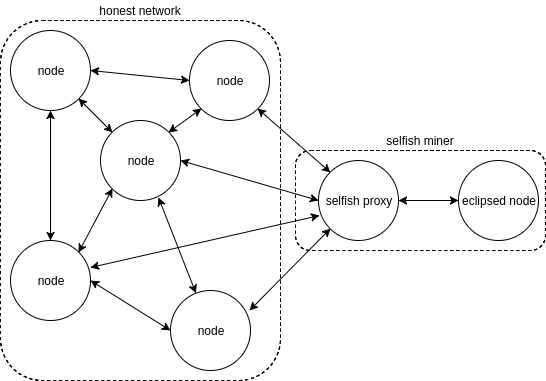
\includegraphics[width=10cm]{selfish_proxy}
    \caption{Selfish proxy eclipsing a normal node}
    \label{fig:selfish_proxy}
\end{figure}

The implementation of all network related functionalities of the selfish proxy is based on the two open-source libraries \textit{pycoin} \cite{pycoin} and \textit{python-bitcoinlib} \cite{python-bitcoinlib}.
The library \textit{pycoin} provides simple networking utilities to connect to other \textit{Bitcoin} nodes and to manage those connections. 
The \textit{python-bitcoinlib} library on the other hand implements functionalities to serialise and de-serialise \textit{Bitcoin} network messages.

\section{Chain}

The selfish proxy continuously collects all block and block headers sent by the connected peers and reassembles the whole chain locally.
To execute the selfish mining algorithm efficiently the proxy needs to retrieve updates of the private and public chain as fast as possible.
Therefore the proxy uses solely block headers to update the chain despite using whole blocks.
The block headers which contain all necessary information to updated the chain can be retrieved faster than the full block because they are just a part of the block and hence smaller.
Furthermore, it is secure for the proxy to trust in the validity of the block header since all other nodes in the network are assumed to behave honestly in our simulation and hence are sending only valid block headers.

When the selfish proxy tries to update the chain with a so far unknown block header, it simply looks at the hash of the previous block stored in the block header.
If the previous block hash is in the chain, the newly received block header is appended to the chain.
On a programmatic level, the proxy uses for that a one-way linked list with the possibility to navigate to the previous block.
In the case the block header has no direct ancestor in the current chain, the header gets preserved as an orphan block.
All orphan blocks are checked on every successful insertion of a block if they now can be added to the chain.

Alongside the information stored in the block, the proxy also keeps track of the block origin and a boolean variable called \textit{transfer\_allowed}. 
The block origin is a simple enumeration if the block was received from the honest network or from the eclipsed node and hence does not change over time.
The \textit{transfer\_allowed} variable determines if the transfer of a block is allowed and is initially always set to \textit{False}.
Depending on the selfish mining strategy the block may be relayed to the other nodes at some later point in time changing the boolean to \textit{True}.
These two variables are stored to be able to distinguish between the public chain, the current longest chain known to the honest network and the private chain, the current longest chain known to  the eclipsed node.
For example to determine the current private chain all blocks originated by the eclipsed node and all blocks with \textit{transfer\_allowed} set to \textit{True} are used.
The two views of the chain are essential for the selfish mining algorithm to decide which action to take and hence when to relay which block to the other side of the network.

\begin{figure}
	\centering
    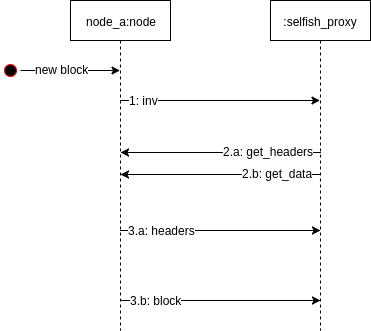
\includegraphics[width=7cm]{receive_block}
    \caption{Selfish proxy receiving a block from another node}
    \label{fig:receive_block}
\end{figure}

\section{Receiving blocks}
\label{chap:receiving_blocks}

An essential capability of the selfish proxy is to retrieve blocks and block headers from its peers.
Figure \ref{fig:receive_block} depicts the communication flow between an arbitrary node called \textit{node\_a} and the selfish proxy which wants to retrieve the information of a new block.
Firstly \textit{node\_a} either finds a new block itself or retrieves a new block from some other node in the network.
Then, adhering to the \textit{Bitcoin} protocol, the node sends an \textit{inv} message (1) containing the hash of the block to its peers including the proxy.
The proxy subsequently checks if it already requested the block from another node or even has the block in the own local chain.
In this two cases, the proxy would just ignore the received hash, and the communication flow would end.
If the block hash is unknown, the proxy sends a \textit{get\_headers} (2.a) message and a \textit{get\_data} (2.b) message to the \textit{node\_a} as pictured in figure \ref{fig:receive_block}.

The \textit{get\_headers} message (2.a) sent by the proxy is composed with an array called block locator hashes and is used to retrieve all block headers after the known block hashes denoted in the array.
To create the array the proxy uses either the private or the public chain depending if \textit{node\_a} is the eclipsed node or a node of the honest network.
The proxy adds then the highest, 2nd, 4th, 8th and 16th highest blocks of the selected chain to the array.
If the chain does not provide all needed bocks, then only the available blocks are added to the block locator array.
\textit{Node\_a}, after it received the \textit{get\_headers}, will search the block hashes from the block locator array in its own longest chain starting with the highest block.
Once a block hash matches a block in the longest chain of \textit{node\_a}, \textit{node\_a} collects all block headers after the matched block in a \textit{headers} message and sends the message back to the proxy (3.a).
In the normal case the proxy trails just one block behind the highest block known by \textit{node\_a}, hence the headers message will contain only one single block header.
In the usual cases the proxy actually felt more then one block behind and \textit{node\_a} will send multiple block headers back to the proxy.
Since the proxy only needs block headers to update the chain, it can immediately update with the received headers the whole chain to the newest tip known tho the \textit{node\_a}.

The \textit{get\_data} message (2.b) sent by the proxy just contains the block hash of the desired block.
As soon as the \textit{node\_a} receives the request for the block, it will return the full block in a \textit{block} message (3.b) to the node.
The request for the whole block lasts typically longer than the request for the newest block headers with the \textit{get\_headers} message as it is pictured in figure \ref{fig:receive_block}.
The proxy request the full block containing all information solely to be able to respond to \textit{get\_data} request by other nodes when it advertises the block on later point in time.

\begin{figure}
	\centering
    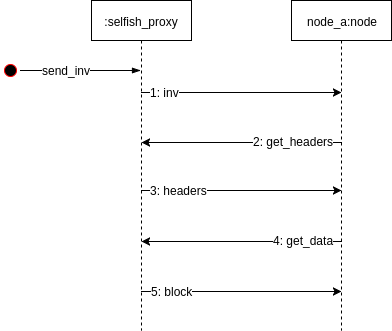
\includegraphics[width=7.5cm]{send_block}
    \caption{Selfish proxy sending a block to another node}
    \label{fig:send_block}
\end{figure}

\section{Sending blocks}
\label{chap:sending_blocks}

After the execution of the selfish mining algorithm, the proxy may want to send a block to the opposite origin of the block.
Figure \ref{fig:send_block} shows the communication flow between an arbitrary \textit{node\_a} and the selfish proxy which intends to relay a block.
The proxy therefore firstly sends the block hash as \textit{inv} message (1) to the \textit{node\_a}.
The \textit{node\_a} after receiving the \textit{inv} message will then reply with a \textit{get\_headers} message (2) because it has not seen the withheld block so far.
The \textit{get\_headers} message contains, similar to the \textit{get\_headers} build by the proxy when it receives a block, known block hashes by \textit{node\_a}.
The proxy then selects either the private or the public chain depending if \textit{node\_a} is the eclipsed node or a node of the honest network.
In the case that there is no unique, longest chain the selfish proxy prefers the chain where the origin of the highest block is the eclipsed node to promote the blocks of the eclipsed node.
Subsequently, the proxy iterates over the selected chain until a block hash from the locator array send by the \textit{node\_a} matches.
The proxy then returns all headers of the blocks after the matched block until the highest block composed in a \textit{headers} message (3).
Afterwards, the \textit{node\_a} will iterate over the received headers and request all missing blocks.
In the usual case, \textit{node\_a} will just lack one block which the node will simply request by sending a \textit{get\_data} message (4) to the proxy.
The selfish proxy replies to this message then by sending a \textit{block} message (5) containing the full block.
Since the selfish mining algorithm already processes the block header before the whole block is available, it could be the case that a block requested by a node is not yet available.
In this case, the proxy defers the reply to the node until it receives the entire block from another node.

\begin{figure}[t]
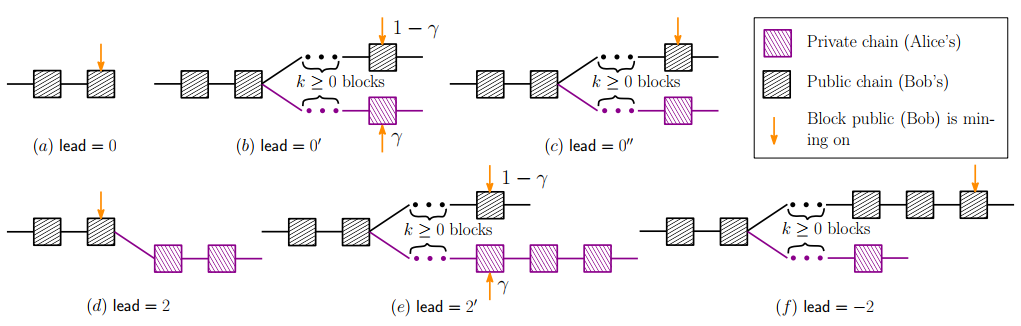
\includegraphics[width=15cm]{private_lead}
\centering
\caption{Different possible leads of the private chain \cite{nayak2016stubborn}}
\label{fig:private_lead}
\end{figure}

\section{Selfish mining}

The selfish proxy executes selfish mining in collaboration with an eclipsed node which is only connected to the proxy as shown in figure \ref{fig:selfish_proxy}.
During the simulation, the proxy monitors the honest network which works on the public chain and the eclipsed node which works on the private chain and performs selfish mining by withholding the blocks created by both sides.

\subsection{Private lead}

Every time a block header is inserted in the chain the proxy checks if either the public or private chain was altered.
In the case that one of these two chains changed the proxy executes the configured selfish mining algorithm.
To easier track the changes between the two chains an integer variable called private lead is used which describes the distance between the two tips of the chain as shown in figure \ref{fig:private_lead}.
A positive lead \textit{n} denotes an advantage of \textit{n} blocks of the private chain over the chain of the honest network.
Conversely, a negative lead \textit{n} stands for a \textit{n} block lag of the eclipsed node over the public chain.
Furthermore, there exist positive leads annotated with an apostrophe denoting that at the height of the public chain a block race happens.
In this block race the possibility that the private chain is extended on the height of the public chain is $\gamma$ and the probability that the public chain gets extended is $1 - \gamma$.
Lastly, a private lead of zero can be annotated with two apostrophes expressing that both chains have the same height but everyone is mining on his own chain.

\subsection{Actions}

The execution of the algorithm outputs one of the four possible actions \textit{adopt}, \textit{override}, \textit{match} and \textit{wait} equivalent defined in the work of \cite{sapirshtein2016optimal}.
An action describes which blocks should be advertised and relayed to the other side of the network at a given point in time:

\begin{itemize}
	\item \textbf{Adopt}: 
	The action \textit{adopt} means that the selfish miner adopts the chain of the honest network. 
	This is a typical action if the private lead is zero and the honest network finds a new block. 
	Then it can be sensitive to just adopt to this new block.
	To execute the \textit{adopt} action the selfish proxy relays the public chain to the eclipsed node by advertising unknown, public blocks.
	\item \textbf{Override}:
	The \textit{override} action is only possible if the private lead is greater then zero after the insertion of the new block header.
	In this case, the selfish proxy can override the public chain by sending out the private blocks mined by the eclipse node.
	Hence, when the proxy executes the \textit{override} action, it sends all private blocks including the first block strictly higher than the public chain.
	If there are even higher private blocks, the selfish proxy keeps them back for further selfish mining.
	\item \textbf{Match}:
	The \textit{match} action is only feasible if the private lead previous the insertion of the block header was greater than zero and the origin of the block is the honest network.
	In this case, the selfish proxy can advertise the private block at the same height to the honest network creating a block race.
	After the execution of the \textit{match} action, the resulting private lead is annotated with an apostrophe to denote the block race.
	\item \textbf{Wait}:
	If the selfish algorithm outputs the \textit{wait} action, then the proxy does simply nothing and waits for the next block which changes either the private or the public chain.
\end{itemize}

\begin{figure}[t]
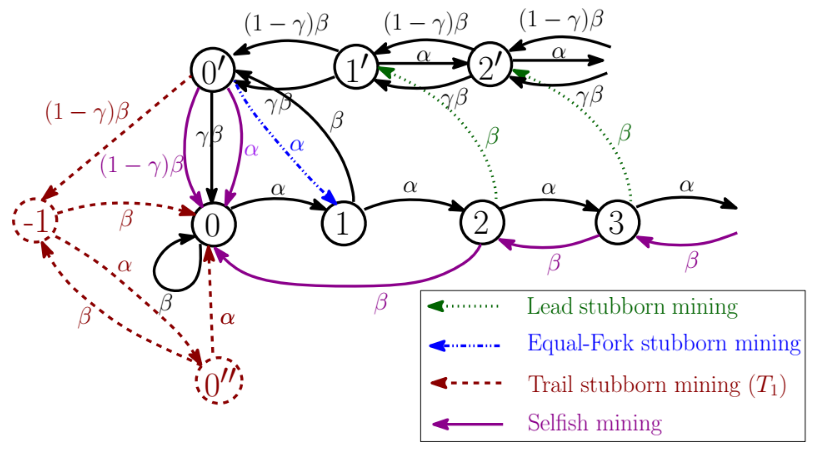
\includegraphics[width=10cm]{stubborn_mining}
\centering
\caption{Categorization of different mining strategies \cite{nayak2016stubborn}}
\label{fig:stubborn_mining}
\end{figure}

\subsection{Strategies}

The selfish mining strategies are defining which action the algorithm implemented in the proxy should execute after a new block was found in the network.
All strategies implemented in the proxy are based on the selfish mining strategy described by \cite{eyal2014majority} (abbreviated with \textit{H}) and can be modified with the three modifications lead (\textit{L}), equal-fork (\textit{F}) and trail stubborn (\textit{T}) by \cite{nayak2016stubborn}.
Figure \ref{fig:stubborn_mining} shows all strategies as a state machine where the label of the states stands for the private lead.
The labels $\alpha$ and $\beta$ used in the transitions are describing the probability that either the eclipsed node or the honest network finds a block.
The variable $\gamma$ represents the likelihood that the part of the honest network which mines on the private chain finds a block.

In the normal selfish mining strategy two possible cases can occur in state \textit{0}.
If the honest network finds a block, then the selfish miner immediately adopts to the public chain and hence remains in the state \textit{0}.
In the other case where the selfish miner finds a block, the state 1 is reached because the selfish miner does not share the block with the honest network.
The same happens if the selfish miner finds more blocks.
Then the selfish miner simple does not share his blocks advancing to state \textit{2} and onwards.
In state \textit{1} the selfish miner has a private lead of one block.
If then the honest network honest network finds a block the selfish miner immediately releases the private block and starts a block race.
Any node in the honest block either chooses the private-public or the public block to mine on top depending which block it sees first.
The block race is dissolved after any node in the network finds a block.
If the honest network finds a block, then the selfish miner adopts to the new tip.
In the other case where the selfish miner finds a block it immediately sends out the block to win the race.
In both cases, the state \textit{0} is reached again.
Lastly, if the private lead is two and the honest network finds a block then the selfish miner immediately publishes the two blocks.
This overrides the newly created block by the honest network, and the state \textit{0} is reached.

As introduced by \cite{nayak2016stubborn} the selfish mining strategy can be modified as follows:

\begin{itemize}
	\item \textbf{Lead stubborn mining (\textit{L})}:
	In lead stubborn mining, the selfish miner tries to cause as many block races as possible.
	So whenever the private chain is longer than the public chain, and the honest network finds a block the selfish miner releases the competing block with the same high causing a block race.
	This behaviour is also applied in state \textit{2} where the selfish miner overwrites typically the block appended to the public chain by publishing two blocks.
	In lead stubborn mining, the selfish miner only releases the competing block an starts a block race denoted with the state \textit{2'}.
	This strategy is promising when $\gamma$ is high implying that whenever a block race occurs, it is likely that the honest network finds a block on published block of the selfish miner. 
	Hence, the honest network unwillingly helps the selfish miner to succeed the private chain during the block race.
	\item \textbf{Equal-fork stubborn mining (\textit{F})}:
	The equal-fork stubborn mining strategy changes the behaviour of the selfish miner during a block race in state \textit{0'}.
	Usually, the selfish miner would use the created block to overwrite the public chain hence winning the block race.
	Using the equal-fork stubborn strategy, the miner keeps the block back which leads to state \textit{1} and the honest network remains mining on two different tips of the chain.
	Thus the strategy compromises the idea to keep the honest network split over two chains as long as possible.
	\item \textbf{Trail stubborn mining (\textit{T})}:
	In trail stubborn mining, the selfish miner allows the private chain to even trail behind the public chain.
	If the block race in state \textit{0'} is won by the honest network, the selfish miner does not adopt the public chain and trails back leading into state \textit{-1}.
	In the case that the selfish miner can catch up by creating a new block the state \textit{0''} where both chains have the same length.
	The trail stubborn strategy finally pays off when the selfish miner finds another block and can override the public chain with the private chain.
	Trail stubbornness is parametrised with an integer \textit{n} determining how many blocks the private chain is allowed to trail behind the public chain.
	If this threshold is reached the selfish miner dismisses his private chain and adopts to the public chain by reaching again state \textit{0}.
\end{itemize}

The modifications of the selfish mining strategy can lead to even more relative gain for the selfish miner depending on the actual computational share and the parameter $\gamma$.
Furthermore, the strategies can be combined and since the trail stubbornness can be parametrised the build an infinite strategy space.

Furthermore, the strategies can be combined and since the trail stubbornness can be parametrized the build an infinite strategy space

\subsection{Algorithm}

The selfish mining strategies and its modifications are implemented in selfish proxy by a simple algorithm using normal control flow structures.
Since the selfish proxy does not have a holistic overview of when a node finds a block, it only can try to apply selfish mining whenever the public or private chain changes locally after the insertion of a new block header.
The algorithm mimics the behaviour shown in the state diagram from figure \ref{fig:stubborn_mining} by looking at the private lead before the insertion of the block header and the origin of the inserted block header.
For example, if the private lead before the insertion of the block header was one and the block header was appended to the public chain.
This would correspond to the state \textit{1} and the outgoing transition $\beta$ which leads in the state diagram to the state \textit{0'} denoting a block race.
The selfish mining algorithm must now assure that this state is also reached in the simulated network by starting a block race.
Thus the algorithm needs to execute the \textit{match} action by publishing the private block to the honest network.

Listing \ref{lst:algo} shows a part of the algorithm, namely the part where the private lead before the insertion is 0, and an action to be executed is searched.
Hence, this part of the algorithm reflects the states 0, 0' and 0'' of the state machine pictured in figure \ref{fig:selfish_mining}.
In the lines 2 to 6, the state 0 is treated by simply looking at the origin of the last block.
If the block was mined by the honest network, then the proxy just adopts to the public chain.
In the other case, the block was found by the eclipsed node, and the proxy just waits for the next block to be discovered.

The lines 7 to 17 are covering the 0' and 0'' states.

\begin{minipage}{\linewidth}
\begin{lstlisting}[caption=Part of the selfish mining algorithm where private lead is zero, label={lst:algo}, basicstyle=\ttfamily, captionpos=b]
if private_lead == 0:
    if length_private == 0:
        if last_block_origin is BlockOrigin.public:
            return Action.adopt
        else:
            return Action.wait
    else:
        if last_block_origin is BlockOrigin.public:
            if self.trail_stubborn < 0:
                return Action.wait
            else:
                return Action.adopt
        else:
            if self.active and self.equal_fork_stubborn:
                return Action.wait
            else:
                return Action.override
\end{lstlisting}
\end{minipage}

In the case the last block was found by the honest network, the proxy adopts to the public chain except the algorithm was configured with trail stubbornness.
Then the proxy waits and hopes to catch up with the public chain at a later point (line 10).
The other case, implemented from line 7 to 17, reflects the fact when the block is found by the eclipsed node.
Then normally the proxy would override the chain by sending the respective private blocks to the honest network.
An exception to this is when currently a block race is happening, and the algorithm is configured with equal-fork stubbornness.
In that case, the selfish algorithm currently has set the variable \textit{active} to \textit{True} and applies equal-fork stubbornness by executing the \textit{wait} action.

\subsection{Configuration}

The selfish proxy started with any configuration executes the standard selfish mining strategy with no modifications.
On execution time the three modifications lead, equal-fork and trail stubborn mining can be configured by using input arguments:

\begin{itemize}
	\item \textit{lead\_stubborn}:
	A boolean input argument determining if lead stubbornness should be used. 
	\item \textit{equal\_fork\_stubborn}:
	A boolean input argument defining if equal-fork stubbornness should be applied or not.
	\item \textit{trail\_stubborn}:
	Used with an integer specifying how much the selfish proxy should trail back.
\end{itemize}
